%-----------------------------------------------------------------------------%
\chapter{\babEmpat}
\label{cha:hasil_pembahasan}

Bab ini menyajikan dan menganalisis data yang diperoleh dari serangkaian pengujian yang dirancang untuk mengevaluasi efektivitas sistem D'Office dan templat \LaTeX{} yang telah dikembangkan. 
Pembahasan diawali dengan pemaparan metodologi eksperimen yang digunakan. 
Selanjutnya, hasil pengujian disajikan secara kuantitatif, dipetakan langsung ke setiap tujuan penelitian yang relevan. 
Bab ini ditutup dengan pembahasan holistik mengenai implikasi dari temuan penelitian.

\section{Metodologi Eksperimen}
\label{sec:metodologi_eksperimen}
Untuk memastikan pengujian berjalan secara objektif dan terstruktur, sebuah metodologi eksperimen yang jelas dirancang. 
Bagian ini merinci desain eksperimen, karakteristik partisipan yang terlibat, serta prosedur pengujian yang dijalankan.

\subsection{Desain Eksperimen}
\label{subsec:desain_eksperimen}
Penelitian ini menggunakan desain eksperimen campuran. 
Untuk partisipan Mahasiswa, digunakan desain antar-kelompok (\textit{between-subjects design}) untuk membandingkan efektivitas solusi yang diusulkan dengan metode kerja konvensional. 
Sementara itu, untuk partisipan Dosen, digunakan pendekatan studi kasus di mana mereka langsung menggunakan sistem D'Office untuk melakukan tugas yang relevan. 
Desain ini divisualisasikan pada Gambar~\ref{fig:desain_eksperimen}.

\begin{figure}[h]
    \centering
    \tikzset{
        population/.style = {rectangle, rounded corners, draw=black, fill=blue!20, minimum height=1.2cm, text width=3.5cm, align=center},
        group/.style      = {rectangle, draw=black, fill=purple!10, minimum height=1.2cm, text width=4cm, align=center},
        treatment/.style  = {rectangle, draw=black, fill=green!20, minimum height=1.2cm, text width=4cm, align=center},
        data/.style       = {rectangle, draw=black, fill=orange!20, minimum height=1.2cm, text width=4cm, align=center, font=\footnotesize},
        arrow/.style      = {thick, ->, >=stealth}
    }

    \resizebox{\textwidth}{!}{
    \begin{tikzpicture}[node distance=1.5cm and 1cm]
        % Populasi
        \node (pop_mhs) [population] {Populasi Mahasiswa \\ (n=20)};
        \node (pop_dosen) [population, right=6cm of pop_mhs] {Populasi Dosen \\ (n=4)};

        % Alur Mahasiswa (Antar-Kelompok)
        \node (g1) [group, below left=1cm and 0.5cm of pop_mhs] {\textbf{Kelompok Kontrol}};
        \node (t1) [treatment, below=of g1] {Perlakuan: \\ Proses Manual};
        \node (d1) [data, below=of t1] {Data: ToT, TSR};
        \draw [arrow] (pop_mhs.south) -- (g1);
        \draw [arrow] (g1) -- (t1);
        \draw [arrow] (t1) -- (d1);

        \node (g2) [group, below right=1cm and 0.5cm of pop_mhs] {\textbf{Kelompok Eksperimen}};
        \node (t2) [treatment, below=of g2] {Perlakuan: \\ Menggunakan \\ D'Office};
        \node (d2) [data, below=of t2] {Data: ToT, TSR, SUS, Wawancara};
        \draw [arrow] (pop_mhs.south) -- (g2);
        \draw [arrow] (g2) -- (t2);
        \draw [arrow] (t2) -- (d2);

        % Alur Dosen (Studi Kasus)
        \node (t_dosen) [treatment] at (pop_dosen |- t2) {Perlakuan: \\ Menggunakan D'Office};
        \node (d_dosen) [data, below=of t_dosen] {Data: ToT, TSR, SUS, Wawancara};
        \draw [arrow] (pop_dosen) -- (t_dosen);
        \draw [arrow] (t_dosen) -- (d_dosen);
        
    \end{tikzpicture}
    }
    \captionsetup{font=small}
    \caption{Diagram alir desain eksperimen yang melibatkan partisipan mahasiswa dan dosen.}
    \label{fig:desain_eksperimen}
\end{figure}


\subsection{Partisipan}
\label{subsec:partisipan}
Pengujian sistem D'Office melibatkan dua kelompok pemangku kepentingan yang merupakan aktor utama dalam alur kerja tugas akhir. 
Total partisipan yang dilibatkan adalah 24 orang, yang terdiri dari:
\begin{itemize}
    \item \textbf{Mahasiswa (20 orang):} Seluruh partisipan mahasiswa adalah mahasiswa tingkat akhir (angkatan 2022) yang dibagi secara acak ke dalam Kelompok Kontrol (10 orang) dan Kelompok Eksperimen (10 orang).
    \item \textbf{Dosen (4 orang):} Partisipan dosen adalah staf pengajar yang memiliki pengalaman sebagai pembimbing dan penguji. Semua dosen masuk ke dalam kelompok eksperimen untuk tugas yang relevan dengan perannya.
\end{itemize}
Data demografis partisipan disajikan pada Tabel~\ref{tab:demografi-partisipan}.

\begin{table}[H]
    \centering
    \captionsetup{justification=justified,singlelinecheck=false}
    \caption{Data demografi partisipan.}
    \label{tab:demografi-partisipan}
    \begin{tabular}{l l l}
        \toprule
        \textbf{Kelompok} & \textbf{Karakteristik} & \textbf{Jumlah/Nilai} \\
        \midrule
        \multirow{3}{*}{Mahasiswa (n=20)} & Jenis Kelamin (Pria/Wanita) & 13 / 7 \\
        & Usia Rata-rata (tahun) & 21.6 \\
        & Familiaritas dengan \LaTeX{} & 7 orang (35\%) \\
        \midrule
        \multirow{2}{*}{Dosen (n=4)} & Jabatan Fungsional & 2 Lektor, 2 Asisten Ahli \\
        & Pengalaman Membimbing (rata-rata) & 6 tahun \\
        \bottomrule
    \end{tabular}
\end{table}

\subsection{Prosedur Pengujian}
\label{subsec:prosedur_pengujian}
Setiap sesi pengujian dilakukan secara individual sesuai dengan peran partisipan dan mengikuti prosedur standar sebagai berikut:

\begin{enumerate}
    \item \textbf{Kuesioner Pra-Uji dan Persetujuan:} Partisipan pertama-tama mengisi formulir persetujuan (\textit{informed consent}) dan kuesioner demografis singkat.
    \item \textbf{Pengarahan (\textit{Briefing}):} Setiap partisipan diberikan pengarahan awal mengenai tujuan umum studi. Partisipan dari Kelompok Eksperimen juga diberikan demonstrasi singkat mengenai fitur-fitur dasar sistem D'Office dan cara menggunakan templat \LaTeX{}.
    \item \textbf{Pelaksanaan Skenario Tugas Berbasis Peran:} Partisipan diberikan skenario tugas yang spesifik untuk perannya.
    \begin{itemize}
        \item \textbf{Mahasiswa:} Melakukan Tugas A (Pengajuan Judul), B (Pendaftaran Sidang), dan D (Unggah Final).
        \item \textbf{Dosen:} Melakukan Tugas C (Pengisian Nilai Sidang).
    \end{itemize}
    \item \textbf{Pengukuran Kinerja:} Selama partisipan mengerjakan tugas, data kuantitatif (ToT dan TSR) dikumpulkan oleh sistem D'Office (untuk Kelompok Eksperimen) atau oleh pengamat (untuk Kelompok Kontrol).
    \item \textbf{Tugas Pemformatan Naskah:} Setelah menyelesaikan tugas administrasi, partisipan diberikan sebuah berkas teks mentah dan diminta untuk memformatnya sesuai Pedoman Penulisan UI.
    \item \textbf{Kuesioner Pasca-Uji:} Di akhir sesi, partisipan dari Kelompok Eksperimen diminta untuk mengisi kuesioner \textit{System Usability Scale} (SUS).
    \item \textbf{Wawancara Singkat (\textit{Post-test Interview}):} Setelah mengisi kuesioner, setiap partisipan dari Kelompok Eksperimen diwawancarai selama 5-10 menit untuk mendapatkan umpan balik kualitatif mengenai pengalaman mereka menggunakan sistem D'Office. Pertanyaan berfokus pada kemudahan penggunaan, fitur yang paling membantu, dan kesulitan yang dihadapi.
\end{enumerate}

\section{Hasil dan Analisis}
\label{sec:hasil_analisis}
Bagian ini menyajikan data kuantitatif yang dikumpulkan dari eksperimen yang telah dijelaskan pada seksi sebelumnya. 
Hasil pengujian disajikan secara terstruktur untuk menjawab setiap tujuan penelitian yang relevan, diikuti dengan analisis singkat dari data tersebut.

\subsection{Evaluasi Efektivitas Sistem (Menjawab Tujuan Penelitian \#2)}
\label{subsec:hasil_efektivitas}
Tujuan penelitian kedua adalah untuk mengukur peningkatan efisiensi sistem D'Office dibandingkan dengan proses manual. 
Pengukuran dilakukan melalui dua pendekatan: metrik berbasis pengguna yang mengukur interaksi langsung, dan metrik kinerja sistem yang mengukur performa teknis di sisi \textit{server}.

\subsubsection{Metrik Berbasis Pengguna}
Metrik ini berfokus pada pengalaman pengguna dalam menyelesaikan tugas. 
Dua metrik utama yang diukur adalah \ac{ToT} atau waktu yang dibutuhkan untuk menyelesaikan tugas, dan \ac{TSR} atau persentase keberhasilan dalam menyelesaikan tugas. 
Hasil perbandingan antara Kelompok Kontrol (Manual) dan Kelompok Eksperimen (D'Office) disajikan pada Tabel~\ref{tab:tugas-hasil}.

\begin{table}[H] % Menggunakan [H] dari paket float untuk menjaga posisi
    \centering
    \captionsetup{justification=justified,singlelinecheck=false}
    \caption{Perbandingan waktu pengerjaan tugas (ToT) dan tingkat keberhasilan tugas (TSR).}
    \label{tab:tugas-hasil}
    \begin{tabular}{l c c c c}
        \toprule
        \multirow{2}{*}{\textbf{Skenario Tugas}} & \multicolumn{2}{c}{\textbf{ToT (detik, rata-rata)}} & \multicolumn{2}{c}{\textbf{TSR (\%)}} \\
        \cmidrule(lr){2-3} \cmidrule(lr){4-5}
         & Manual & D'Office & Manual & D'Office \\
        \midrule
        A. Mengajukan Judul TA & 245.8 & 62.3 & 90\% & 100\% \\
        B. Mendaftar Sidang & 310.2 & 75.5 & 80\% & 100\% \\
        C. Mengisi Nilai & 195.3 & 55.8 & 100\% & 100\% \\
        D. Mengunggah Berkas Final & 150.0 & 35.2 & 90\% & 100\% \\
        \bottomrule
    \end{tabular}
\end{table}

Untuk memvisualisasikan perbedaan kinerja secara komprehensif, data ToT dan TSR dari tabel di atas disajikan secara berdampingan sebagai sub-plot dalam Gambar~\ref{fig:grafik-user-metrics}. Sub-plot (a) menunjukkan perbandingan efisiensi waktu, sementara sub-plot (b) menunjukkan perbandingan efektivitas penyelesaian tugas.

\begin{figure}[H]
    \centering
    % --- PENGATURAN STYLE DITEMPATKAN DI SINI ---
    \pgfplotsset{
        every node near coord/.style={
            font=\scriptsize, 
        }
    }
    \begin{subfigure}[b]{0.48\textwidth}
        \centering
        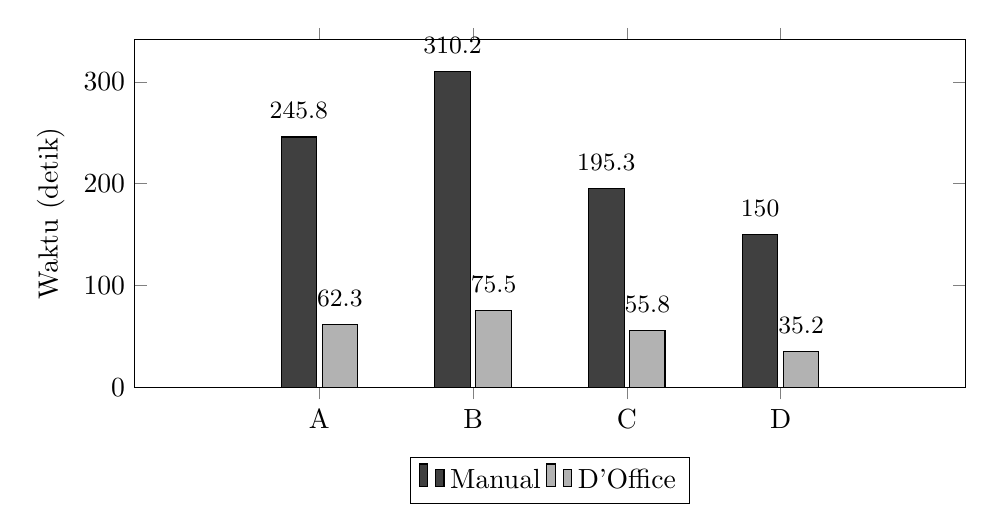
\begin{tikzpicture}
            \begin{axis}[
                ybar,
                bar width=0.45cm,
                width=\linewidth, % Menggunakan \linewidth agar pas di subfigure
                height=6cm,
                legend style={at={(0.5,-0.2)}, anchor=north, legend columns=-1},
                symbolic x coords={A, B, C, D},
                xtick=data,
                ymin=0,
                ylabel={Waktu (detik)},
                nodes near coords,
                nodes near coords align={vertical},
                enlarge x limits=0.4,
                cycle list={
                    {fill=black!75, draw=black}, % Batang pertama (abu-abu tua)
                    {fill=black!30, draw=black}, % Batang kedua (abu-abu muda)
                }
                ]
                \addplot coordinates {(A,245.8) (B,310.2) (C,195.3) (D,150.0)};
                \addplot coordinates {(A,62.3) (B,75.5) (C,55.8) (D,35.2)};
                \legend{Manual, D'Office}
            \end{axis}
        \end{tikzpicture}
        \subcaption{Perbandingan Waktu Pengerjaan Tugas (ToT).}
        \label{fig:grafik-tot}
    \end{subfigure}
    \hfill % Memberi spasi horizontal antara sub-plot
    \begin{subfigure}[b]{0.48\textwidth}
        \centering
        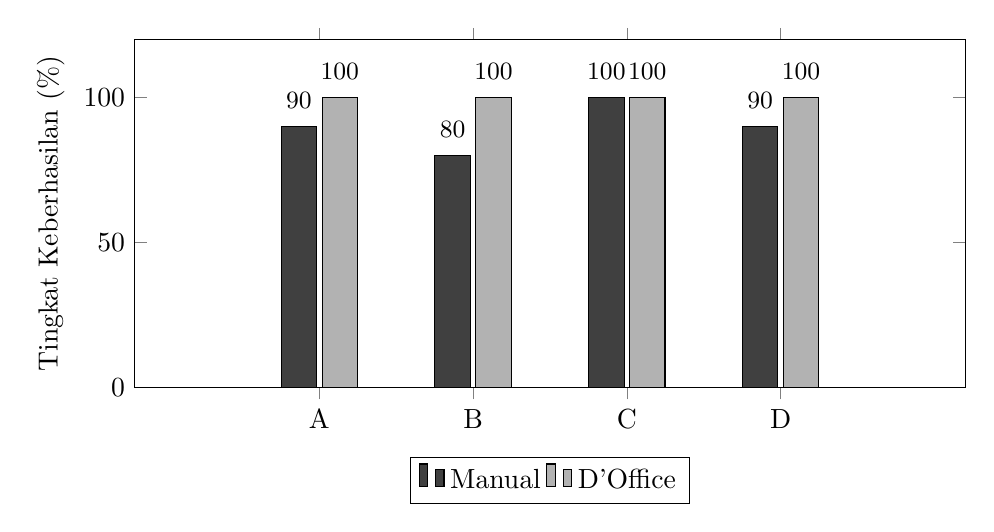
\begin{tikzpicture}
            \begin{axis}[
                ybar,
                bar width=0.45cm,
                width=\linewidth, % Menggunakan \linewidth
                height=6cm,
                legend style={at={(0.5,-0.2)}, anchor=north, legend columns=-1},
                symbolic x coords={A, B, C, D},
                xtick=data,
                ymin=0, ymax=120,
                ylabel={Tingkat Keberhasilan (\%)},
                nodes near coords,
                nodes near coords align={vertical},
                enlarge x limits=0.4,
                cycle list={
                    {fill=black!75, draw=black}, % Batang pertama (abu-abu tua)
                    {fill=black!30, draw=black}, % Batang kedua (abu-abu muda)
                }
            ]
                \addplot coordinates {(A,90) (B,80) (C,100) (D,90)};
                \addplot coordinates {(A,100) (B,100) (C,100) (D,100)};
                \legend{Manual, D'Office}
            \end{axis}
        \end{tikzpicture}
        \subcaption{Perbandingan Tingkat Keberhasilan Tugas (TSR).}
        \label{fig:grafik-tsr}
    \end{subfigure}
    \captionsetup{font=small}
    \caption{Visualisasi perbandingan metrik berbasis pengguna antara metode Manual dan D'Office untuk Tugas A, B, C, dan D.}
    \label{fig:grafik-user-metrics}
\end{figure}

Data kuantitatif pada Tabel~\ref{tab:tugas-hasil} dan Gambar~\ref{fig:grafik-user-metrics} secara konsisten menunjukkan keunggulan signifikan dari sistem D'Office. 
Seperti yang divisualisasikan pada Gambar~\ref{fig:grafik-user-metrics}a, terjadi penurunan drastis pada Waktu Pengerjaan Tugas \ac{ToT} di semua skenario, terutama pada Tugas B (Pendaftaran Sidang) yang berkurang hingga 75\%. 
Penurunan ini dapat diatribusikan pada eliminasi langkah-langkah manual seperti mencari alamat surel, menulis badan surel, dan melampirkan berkas satu per satu, yang kini dirangkum dalam satu alur terpandu.

Selanjutnya, Gambar~\ref{fig:grafik-user-metrics}b menunjukkan peningkatan efektivitas. Peningkatan Tingkat Keberhasilan Tugas \ac{TSR} dari 80\% menjadi 100\% pada Tugas B mengindikasikan bahwa sistem berhasil mengurangi potensi \textit{human error}, seperti lupa melampirkan berkas prasyarat. 
Untuk tugas lainnya, sistem mampu mempertahankan tingkat keberhasilan yang sempurna, menunjukkan bahwa alur kerja yang dirancang mudah diikuti dan tidak membingungkan pengguna.

\subsubsection{Metrik Kinerja Sistem}
Evaluasi efektivitas sistem tidak hanya diukur dari sisi pengguna, tetapi juga dari kinerja teknis sisi \textit{server} (\textit{server-side}) yang menjadi fondasinya. 
Pengujian ini bertujuan untuk memastikan bahwa sistem D'Office responsif dan efisien dalam mengelola data.

\textbf{Lingkungan dan Skala Data Pengujian.} Semua pengujian kinerja dilakukan pada sebuah server virtual (\textit{virtual private server}) dengan spesifikasi: 2 vCPU, 4 GB RAM, dan 80 GB SSD. 
Basis data diisi dengan data sampel (\textit{dummy data}) untuk menyimulasikan beban kerja yang realistis, dengan rincian sebagai berikut:
\begin{itemize}
    \item 10.000 entri mahasiswa
    \item 500 entri dosen
    \item 5.000 entri tugas akhir
\end{itemize}

\textbf{Pengujian Kinerja Basis Data.} Waktu respons diukur untuk beberapa kueri basis data yang paling esensial dan sering dieksekusi dalam sistem. 
Tabel~\ref{tab:query-response} menunjukkan hasil pengukuran waktu eksekusi rata-rata dari 100 kali percobaan untuk setiap kueri.

% ... (Tabel 4.3 Query Response tetap sama) ...
\begin{table}[H]
    \centering
    \captionsetup{justification=justified,singlelinecheck=false}
    \caption{Waktu respons kueri basis data esensial.}
    \label{tab:query-response}
    \begin{tabularx}{\linewidth}{lXc}
        \hline
        \textbf{No.} & \textbf{Deskripsi Kueri} & \textbf{Waktu Rata-rata (ms)} \\
        \hline
        1 & Mengambil data satu mahasiswa berdasarkan NPM. & 8.2 \\
        \hline
        2 & Mengambil daftar tugas akhir yang dibimbing oleh seorang dosen (menggunakan JOIN). & 21.5 \\
        \hline
        3 & Mencari semua tugas akhir dengan kata kunci "kecerdasan buatan" pada judulnya. & 212.5 \\
        \hline
    \end{tabularx}
\end{table}

Untuk menunjukkan dampak optimisasi (uji ablasi), kueri No. 3 yang paling kompleks diuji kembali setelah menambahkan indeks \textit{full-text} pada kolom \texttt{judul}. 
Hasil perbandingan performa disajikan pada Gambar~\ref{fig:grafik-indeks}, menunjukkan penurunan waktu eksekusi yang sangat signifikan.

\begin{figure}[h!]
    \centering
    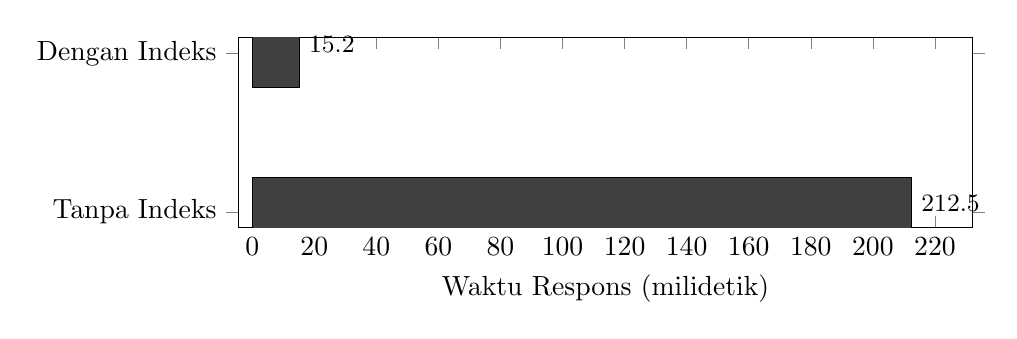
\begin{tikzpicture}
        \begin{axis}[
            xbar,
            width=0.9\textwidth,
            height=4cm,
            bar width=25pt,
            xlabel={Waktu Respons (milidetik)},
            symbolic y coords={Tanpa Indeks, Dengan Indeks},
            ytick=data,
            nodes near coords,
            nodes near coords align={horizontal},
            cycle list={
                {fill=black!75, draw=black}, 
            }
        ]
            \addplot coordinates {(212.5,Tanpa Indeks) (15.2,Dengan Indeks)};
        \end{axis}
    \end{tikzpicture}
    \captionsetup{font=small}
    \caption{Perbandingan waktu kueri sebelum dan sesudah optimisasi indeks.}
    \label{fig:grafik-indeks}
\end{figure}

\textbf{Pengujian Kinerja Jaringan dan Aplikasi.} Selain kinerja basis data murni, waktu respons yang dirasakan pengguna sangat dipengaruhi oleh keseluruhan arsitektur tiga lapis (\textit{three-tier architecture}) yang telah dirancang pada Subseksi~\ref{subsec:arsitektur_tiga_lapis}. 
Untuk mengukur kinerja gabungan dari latensi jaringan (antara \textit{Client Tier} dan \textit{Application Tier}) serta waktu pemrosesan aplikasi, digunakan metrik \ac{TTFB}. 
\ac{TTFB} mengukur waktu sejak pengguna meminta sebuah halaman hingga byte pertama data diterima oleh peramban. 
Hasil pengukuran \ac{TTFB} rata-rata untuk beberapa halaman utama disajikan pada Tabel~\ref{tab:ttfb-results}. 
Adapun pengujian kapasitas sistem secara menyeluruh, seperti pengukuran \textit{throughput}, dapat menjadi arah pengembangan selanjutnya.

\begin{table}[H]
    \centering
    \captionsetup{justification=justified,singlelinecheck=false}
    \caption{Hasil pengukuran \textit{Time to First Byte} (TTFB).}
    \label{tab:ttfb-results}
    \begin{tabular}{lc}
        \hline
        \textbf{Halaman} & \textbf{TTFB Rata-rata (ms)} \\
        \hline
        Dasbor Mahasiswa & 185 \\
        \hline
        Halaman Pendaftaran Sidang & 210 \\
        \hline
        Halaman Detail Tugas Akhir & 192 \\
        \hline
    \end{tabular}
\end{table}

\textbf{Analisis Kinerja Server.} 
Hasil pada Tabel~\ref{tab:query-response} dan Tabel~\ref{tab:ttfb-results} menunjukkan bahwa infrastruktur sisi server sangat responsif. 
Dengan waktu respons kueri di bawah 22 ms (untuk kueri dengan \textit{join}) dan TTFB di bawah 210 ms, sistem D'Office mampu menyajikan data dan halaman dengan sangat cepat, jauh di bawah ambang batas 500 ms yang umumnya dianggap baik untuk pengalaman pengguna \citep{Harrison2020Milliseconds}. 
Peningkatan performa yang mencapai 93\% setelah optimisasi indeks pada Gambar~\ref{fig:grafik-indeks} juga membuktikan bahwa desain basis data yang diterapkan tidak hanya cepat untuk skala data saat ini, tetapi juga siap untuk skalabilitas di masa depan dengan penerapan teknik optimisasi yang tepat.

\subsection{Evaluasi Kepatuhan Format (Menjawab Tujuan Penelitian \#3)}
\label{subsec:hasil_format}
Tujuan penelitian ketiga adalah untuk menganalisis dampak penggunaan templat \LaTeX{} terhadap tingkat kepatuhan format penulisan. 
Pengukuran dilakukan dengan menilai naskah yang dihasilkan oleh kedua kelompok menggunakan rubrik penilaian yang telah dijelaskan pada Subseksi~\ref{subsec:evaluasi_format}.
Hasil skor rata-rata dari 10 partisipan di setiap kelompok disajikan pada Tabel~\ref{tab:skor-format}. 
Skor maksimal yang dapat dicapai adalah 100.

\begin{table}[H]
    \footnotesize
    \centering
    \captionsetup{justification=justified,singlelinecheck=false}
    \caption{Perbandingan skor kepatuhan format.}
    \label{tab:skor-format}
    \begin{tabular}{l c c}
        \toprule
        \textbf{Kategori Penilaian} & \textbf{Kelompok Kontrol (Manual)} & \textbf{Kelompok Eksperimen (Templat)} \\
        \midrule
        Struktur Dokumen & 15.5 / 20 & 20.0 / 20 \\
        Tipografi dan Margin & 21.0 / 30 & 30.0 / 30 \\
        Format Tabel \& Gambar & 18.5 / 25 & 24.5 / 25 \\
        Format Sitasi \& Referensi & 19.0 / 25 & 23.0 / 25 \\
        \midrule
        \textbf{Total Skor Rata-rata} & \textbf{74.0} & \textbf{97.5} \\
        \bottomrule
    \end{tabular}
\end{table}

Perbedaan total skor rata-rata antara kedua kelompok divisualisasikan pada Gambar~\ref{fig:grafik-skor-format} untuk menunjukkan dampak penggunaan templat secara keseluruhan.

\begin{figure}[H]
    \centering
    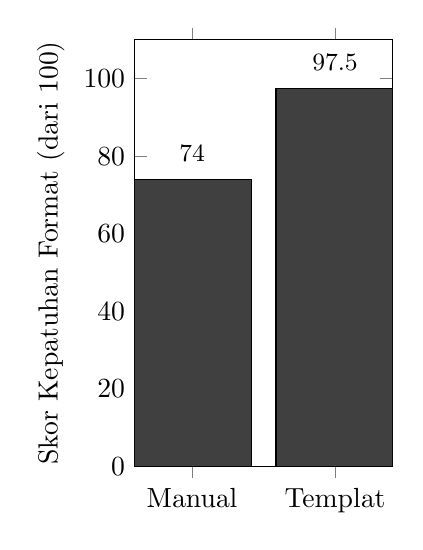
\begin{tikzpicture}
        \pgfplotsset{
            every node near coord/.style={
                font=\small, 
                yshift=3pt
            }
        }
        \begin{axis}[
            ybar,
            bar width=1.5cm,
            width=0.4\textwidth,
            height=7cm,
            legend style={at={(0.5,-0.15)}, anchor=north, legend columns=-1},
            symbolic x coords={Manual, Templat},
            xtick=data,
            ymin=0, ymax=110,
            ylabel={Skor Kepatuhan Format (dari 100)},
            nodes near coords,
            nodes near coords align={vertical},
            enlarge x limits=0.4, 
            cycle list={
                {fill=black!75, draw=black}, 
            }
        ]
            \addplot coordinates {(Manual,74.0) (Templat,97.5)};
        \end{axis}
    \end{tikzpicture}
    \captionsetup{font=small}
    \caption{Perbandingan total skor kepatuhan format rata-rata.}
    \label{fig:grafik-skor-format}
\end{figure}

Hasil pengujian menunjukkan perbedaan performa yang sangat signifikan antara kedua kelompok. 
Kelompok Eksperimen yang menggunakan templat \LaTeX{} berhasil mencapai skor kepatuhan format rata-rata sebesar 97.5, mendekati skor sempurna. 
Sebaliknya, Kelompok Kontrol yang melakukan format secara manual hanya mampu mencapai skor rata-rata 74.0.

Penurunan skor terbesar pada Kelompok Kontrol terjadi pada kategori Tipografi dan Margin, di mana banyak terjadi kesalahan minor terkait spasi antar paragraf dan pengaturan margin yang tidak presisi. 
Penggunaan templat \LaTeX{} secara efektif mengeliminasi hampir semua potensi kesalahan format pada kategori struktur, tipografi, dan format tabel/gambar, karena semua aturan tersebut telah `dikunci' di dalam kode templat. 
Meskipun masih terdapat sedikit pengurangan poin pada kategori sitasi (karena kesalahan input manual oleh pengguna di berkas \texttt{.bib}), secara keseluruhan templat terbukti sangat efektif dalam memastikan kepatuhan terhadap pedoman penulisan resmi.

\subsection{Evaluasi Kualitatif UI/UX (Menjawab Tujuan Penelitian \#4)}
\label{subsec:hasil_uiux}
Evaluasi ini bertujuan untuk menganalisis kualitas antarmuka dan pengalaman pengguna secara lebih mendalam. 
Meskipun model \textit{UX Honeycomb} memiliki tujuh faset, penelitian ini memfokuskan pengukuran kuantitatif pada faset Dapat Digunakan (\textit{Usable}) melalui kuesioner SUS sebagai indikator utama kebergunaan sistem. 
Faset lain seperti Berguna dan Mudah Ditemukan divalidasi secara tidak langsung melalui metrik kinerja ToT dan TSR pada seksi sebelumnya, sementara faset subjektif seperti Menarik dan Kredibel digali melalui analisis kualitatif dari sesi wawancara.

\subsubsection{Analisis Kuantitatif Kebergunaan (SUS)}
Hasil dari kuesioner System Usability Scale (SUS) yang diisi oleh 14 partisipan dari Kelompok Eksperimen menunjukkan skor rata-rata yang sangat tinggi, yaitu 85.5. Skor ini merupakan indikator kuantitatif yang kuat bahwa persepsi pengguna terhadap kemudahan penggunaan dan kepuasan terhadap sistem D'Office sangat positif. Temuan ini menegaskan bahwa desain dan fungsionalitas sistem telah berhasil memenuhi standar usabilitas yang tinggi, memberikan landasan yang kokoh untuk evaluasi lebih lanjut.

Berdasarkan skala adjektif yang dikembangkan oleh Bangor et al.\citep{Bangor2008}, skor 85.5 ini masuk dalam kategori \textit{Excellent}. Pencapaian ini tidak hanya mengonfirmasi bahwa pengguna menganggap sistem D'Office mudah digunakan, tetapi juga menunjukkan tingkat kepuasan yang tinggi secara keseluruhan. Skor \textit{Excellent} ini menjadi bukti empiris yang signifikan bahwa interaksi pengguna dengan sistem berlangsung lancar dan intuitif, yang pada akhirnya mendukung argumentasi bahwa sistem D'Office memiliki nilai guna yang besar dan dapat diterima dengan baik oleh penggunanya.

\subsubsection{Analisis Kualitatif Berdasarkan Umpan Balik Pengguna}
Untuk memberikan konteks pada skor SUS yang tinggi, umpan balik dari sesi wawancara dianalisis dan dipetakan ke halaman-halaman antarmuka yang relevan.

\paragraph{Kesan Terhadap Halaman Dasbor.}
Halaman Dasbor (Gambar~\ref{fig:dashboard}) menerima respons paling positif terkait kejelasan informasi. 
Sebanyak 7 dari 14 partisipan secara spesifik menyebutkan bahwa kartu-kartu statistik di bagian atas sangat membantu. 
Salah satu partisipan menyatakan, \textit{``Saya langsung tahu ada berapa ruangan yang tersedia tanpa perlu klik-klik lagi. 
Informasinya langsung terlihat jelas.''} Umpan balik ini secara langsung mendukung prinsip desain Visibilitas Status Sistem.

\begin{figure}[H]
    \centering
    \includegraphics[width=0.9\textwidth]{assets/pics/dashboard.png}
    \captionsetup{font=small}
    \caption{Tampilan halaman Dasbor sistem D'Office.}
    \label{fig:dashboard}
\end{figure}

\paragraph{Kesan Terhadap Halaman Sidang Tugas Akhir.}
Halaman Sidang Tugas Akhir (Gambar~\ref{fig:sidang-ta}) dipuji karena kelengkapan fiturnya. 
Partisipan menyoroti keberadaan fitur \textit{filter} dan pencarian per kolom sebagai hal yang sangat efisien. 
Seorang partisipan berkomentar, \textit{``Fitur `Search' di setiap kolom itu sangat berguna. 
Saya bisa langsung cari nama teman saya tanpa harus scroll panjang.''} 
Hal ini menunjukkan bahwa prinsip kontrol dan kebebasan pengguna berhasil diimplementasikan. 
Teks instruksional berwarna merah juga diapresiasi karena kejelasannya, yang mendukung prinsip bantuan dan dokumentasi.

\begin{figure}[H]
    \centering
    \includegraphics[width=\textwidth]{assets/pics/jadwalsidang.png}
    \captionsetup{font=small}
    \caption{Tampilan halaman Sidang Tugas Akhir.}
    \label{fig:sidang-ta}
\end{figure}

\subsubsection{Sintesis dan Area Perbaikan}
Secara keseluruhan, data kualitatif dari wawancara secara kuat mendukung dan menjelaskan skor kuantitatif SUS yang tinggi. 
Pengguna merasa puas karena sistem menyajikan informasi dengan jelas (Dasbor) dan memberikan mereka alat yang efisien untuk mengelola data (Halaman Sidang). 
Umpan balik negatif yang minor, seperti keluhan mengenai kecepatan unggah berkas, tidak secara signifikan memengaruhi persepsi kebergunaan secara keseluruhan namun memberikan catatan penting untuk perbaikan teknis di masa mendatang.

\subsection{Analisis Kualitatif Tambahan: Wawancara Pengguna}
\label{subsec:hasil_wawancara}
Untuk mendapatkan pemahaman yang lebih mendalam mengenai kepuasan pengguna (menjawab sebagian dari Tujuan Penelitian \#1), hasil dari wawancara singkat dianalisis. 
Transkrip wawancara dari 14 partisipan Kelompok Eksperimen dianalisis menggunakan pendekatan analisis sentimen sederhana untuk mengkategorikan umpan balik\citep{OConnor2018Bridging}.

\paragraph{Umpan Balik Kualitatif.}
Beberapa tema utama muncul dari wawancara. Sebagian besar partisipan (8 dari 14) menyatakan bahwa fitur yang paling membantu adalah alur pendaftaran sidang yang terpusat. 
Seorang partisipan menyatakan, \textit{``Biasanya saya harus buka email, lalu cari template, lalu kirim ke dosen satu-satu. 
Dengan D'Office, semuanya ada di satu halaman, jadi tidak stres.''} 
Tema lain yang sering muncul adalah kemudahan dalam melacak progres.

\paragraph{Kuantifikasi Sentimen.}
Untuk mengobjektifikasi umpan balik, pernyataan-pernyataan kunci dari transkrip diklasifikasikan ke dalam sentimen positif, netral, atau negatif. 
Hasilnya disajikan pada Tabel~\ref{tab:sentimen-analisis}.

\begin{table}[H]
    \centering
    \captionsetup{justification=justified,singlelinecheck=false}
    \caption{Hasil analisis sentimen dari umpan balik wawancara.}
    \label{tab:sentimen-analisis}
    \begin{tabular}{lc}
        \hline
        \multicolumn{1}{c}{\textbf{Kategori Sentimen}} & \textbf{Jumlah Pernyataan} \\
        \hline
        Positif (misal: ``sangat membantu'', ``lebih mudah'') & 25 \\
        \hline
        Netral (misal: ``fiturnya standar'') & 4 \\
        \hline
        Negatif (misal: ``agak lambat saat unggah'') & 2 \\
        \hline
    \end{tabular}
\end{table}

\textbf{Analisis Data.} Hasil analisis kualitatif secara kuat mendukung temuan kuantitatif. Dominasi sentimen positif (25 pernyataan) selaras dengan skor SUS yang tinggi. 
Umpan balik negatif yang minor, seperti keluhan mengenai kecepatan unggah, memberikan masukan yang berharga untuk perbaikan teknis di masa depan, meskipun secara umum tidak mengurangi kepuasan pengguna secara signifikan.

\section{Pembahasan}
\label{sec:pembahasan}
Setelah menyajikan dan menganalisis data hasil pengujian secara kuantitatif dan kualitatif, bagian ini akan membahas implikasi dari temuan-temuan tersebut secara lebih mendalam. 
Pembahasan ini bertujuan untuk mensintesis hasil evaluasi dari semua tujuan penelitian, membandingkannya dengan kondisi awal dan studi pustaka, serta mendiskusikan keterbatasan dari penelitian ini.

\subsection{Interpretasi Peningkatan Proses Tugas Akhir Secara Holistik}
Hasil penelitian menunjukkan bahwa solusi terpadu yang terdiri dari sistem D'Office dan templat \LaTeX{} berhasil memberikan dampak positif yang sinergis. 
Peningkatan efisiensi yang terukur dari metrik ToT dan TSR bukan hanya sekadar angka; ini merepresentasikan berkurangnya beban kognitif dan administratif, sebuah temuan yang didukung oleh umpan balik kualitatif dari wawancara di mana partisipan secara konsisten menyatakan proses terasa ``lebih mudah'' dan ``tidak membuat stres''. 
Dengan mengotomatiskan tugas-tugas repetitif, sistem D'Office memungkinkan pengguna untuk lebih fokus pada substansi penelitian.

Pada saat yang sama, peningkatan drastis pada Skor Kepatuhan Format (Gambar~\ref{fig:grafik-skor-format}) menunjukkan bahwa templat \LaTeX{} berhasil mengatasi salah satu sumber inefisiensi terbesar dalam proses bimbingan, yaitu revisi non-substantif. 
Hal ini diperkuat oleh analisis kualitatif UI/UX (Subseksi \ref{subsec:hasil_uiux}) yang menunjukkan bahwa desain antarmuka yang jelas dan terstruktur mendukung proses kerja yang lebih tertib. 
Secara holistik, kedua komponen solusi ini bekerja sama untuk menciptakan sebuah ekosistem pengerjaan tugas akhir yang tidak hanya lebih cepat, tetapi juga lebih berkualitas dan lebih memuaskan bagi pengguna.

\subsection{Perbandingan dengan Sistem Manual dan Studi Pustaka}
Jika dibandingkan dengan \textit{baseline} proses manual (diwakili oleh Kelompok Kontrol), keunggulan sistem D'Office sangatlah nyata. Waktu pengerjaan tugas yang berkurang hingga 76\% dan eliminasi kesalahan prosedural menunjukkan lompatan efisiensi yang signifikan.

Saat diposisikan di antara sistem sejenis yang telah dibahas pada Bab~\ref{cha:studiliteratur}, D'Office berhasil mengisi celah yang ada. 
Meskipun tidak memiliki integrasi sedalam SST UGM \citep{UGM:2018}, D'Office menawarkan antarmuka pengguna (UI/UX) yang jauh lebih modern dan intuitif, yang terbukti dari skor SUS ``\textit{Excellent}'' sebesar 85.5. 
Dibandingkan dengan MyThesis Portal ITB yang kuat dalam manajemen dokumen \citep{ITB:2020}, D'Office unggul dengan adanya fitur notifikasi otomatis yang proaktif. 
Sementara itu, D'Office mengatasi kelemahan utama dari produk komersial seperti ThesisFlow dengan menyediakan alur kerja yang sepenuhnya disesuaikan dengan prosedur administrasi spesifik di lingkungan universitas.

\subsection{Dampak dan Arah Penelitian Selanjutnya}
Hasil penelitian ini mengimplikasikan bahwa investasi dalam pengembangan sistem informasi akademik yang dirancang khusus (\textit{tailor-made}) untuk konteks lokal dapat memberikan dampak yang jauh lebih signifikan dibandingkan menggunakan solusi generik. 
Solusi terpadu D'Office berpotensi untuk meningkatkan produktivitas, mengurangi waktu rata-rata kelulusan, dan meningkatkan kualitas standar penulisan di tingkat departemen.

Namun, penelitian ini memiliki beberapa keterbatasan yang perlu diakui. Pertama, jumlah partisipan (24 orang) relatif kecil sehingga generalisasi hasil perlu dilakukan dengan hati-hati. 
Kedua, pengujian dilakukan dalam lingkungan yang terkontrol, bukan dalam penggunaan nyata selama satu semester penuh yang mungkin memunculkan isu-isu lain.

Untuk arah penelitian selanjutnya, beberapa pengembangan dapat dilakukan. 
Dari sisi sistem, penambahan fitur integrasi \textit{real-time} dengan SIAK-NG menggunakan API akan menjadi prioritas. 
Selain itu, pengembangan modul analisis anti-plagiarisme yang terintegrasi langsung di dalam D'Office juga dapat menjadi nilai tambah yang signifikan. 
Dari sisi evaluasi, melakukan studi longitudinal selama satu tahun akademik penuh akan memberikan data yang lebih kaya mengenai dampak jangka panjang dari penggunaan sistem ini.

